\pgfplotsset{compat=1.15}
\usetikzlibrary{arrows}
\definecolor{ffqqqq}{rgb}{1,0,0}
\definecolor{qqqqff}{rgb}{0,0,1}
\definecolor{ffqqff}{rgb}{1,0,1}
\definecolor{xfqqff}{rgb}{0.4980392156862745,0,1}
\definecolor{ududff}{rgb}{0.30196078431372547,0.30196078431372547,1}
\definecolor{yqqqqq}{rgb}{0.5019607843137255,0,0}
\definecolor{qqwwtt}{rgb}{0,0.4,0.2}
\begin{figure}[h!]
\centering
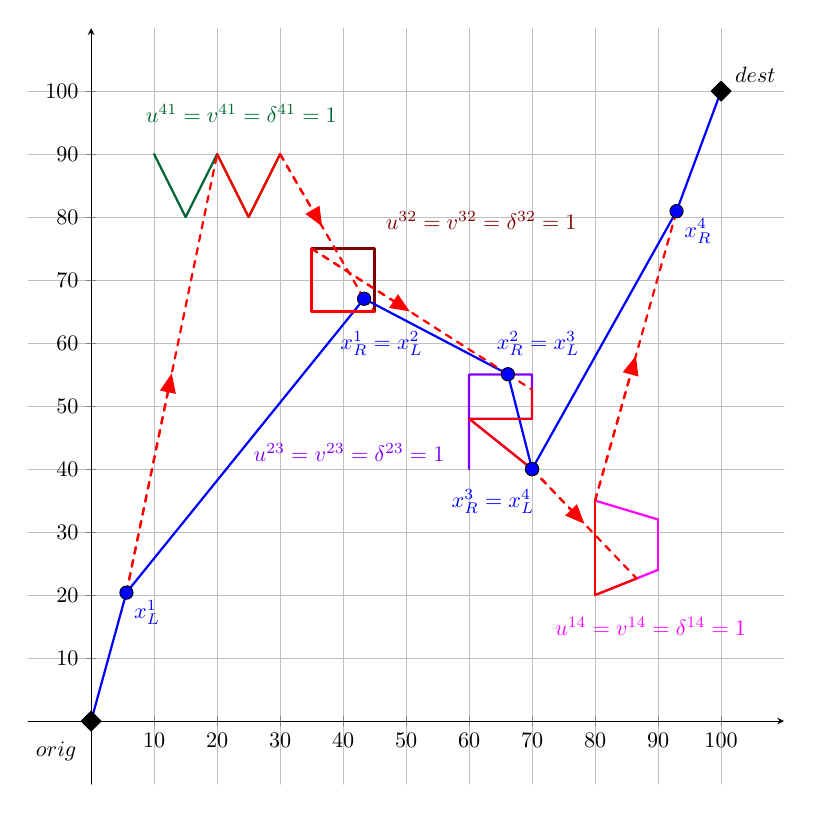
\begin{tikzpicture}[line cap=round,line join=round,>=triangle 45,x=1cm,y=1cm, scale = 0.8]
\begin{axis}[
x=0.1cm,y=0.1cm,
axis lines=middle,
ymajorgrids=true,
xmajorgrids=true,
xmin=-10,
xmax=110,
ymin=-10,
ymax=110,
xtick={0,10,...,100},
ytick={0,10,...,100},]
\clip(-49.903883687724594,-14.69149547687434) rectangle (209.13223427513805,134.7784315983007);
\draw [line width=1pt,color=qqwwtt] (10,90)-- (15,80)-- (20,90)-- (25,80)-- (30,90);
\draw [line width=1pt] (35,75)-- (35,65);
\draw [line width=1pt] (35,65)-- (45,65);
\draw [line width=1pt,color=yqqqqq] (45,65)-- (45,75);
\draw [line width=1pt,color=yqqqqq] (45,75)-- (35,75);
\draw [line width=1pt,color=xfqqff] (60,40)-- (60,55)-- (70,55)-- (70,48)-- (60,48)-- (70,40);
\draw [line width=1pt] (80,35)-- (80,20);
\draw [line width=1pt,color=ffqqff] (80,20)-- (90,24);
\draw [line width=1pt,color=ffqqff] (90,24)-- (90,32);
\draw [line width=1pt,color=ffqqff] (90,32)-- (80,35);
\draw (-10,-2) node[anchor=north west] {$\bm{orig}$};
\draw (101,105) node[anchor=north west] {$\bm{dest}$};
\draw [line width=1pt,color=qqqqff] (0,0)-- (5.6057,20.3868);
\draw [line width=1pt,color=qqqqff] (5.6057,20.3868)-- (43.33,67.04);
\draw [line width=1pt,color=qqqqff] (43.33,67.04)-- (66.16,55.06);
\draw [line width=1pt,color=qqqqff] (66.16,55.06)-- (70,40);
\draw [line width=1pt,color=qqqqff] (70,40)-- (92.93,80.94);
\draw [line width=1pt,color=qqqqff] (92.93,80.94)-- (100,100);
\draw [line width=1pt,dashed,color=ffqqqq] (5.6057,20.3868)-- (20,90);
\draw [line width=1pt,color=ffqqqq] (20,90)-- (25,80);
\draw [line width=1pt,color=ffqqqq] (25,80)-- (30,90);
\draw [line width=1pt,dashed,color=ffqqqq] (30,90)-- (43.33,67.04);
\draw [line width=1pt,dashed,color=ffqqqq] (43.33,67.04)-- (45,65);
\draw [line width=1pt,color=ffqqqq] (45,65)-- (35,65);
\draw [line width=1pt,color=ffqqqq] (35,65)-- (35,75);
\draw [line width=1pt,dashed,color=ffqqqq] (35,75)-- (66.16,55.06);
\draw [line width=1pt,dashed,color=ffqqqq] (66.16,55.06)-- (70,52.5969);
\draw [line width=1pt,color=ffqqqq] (70,52.5969)-- (70,48);
\draw [line width=1pt,color=ffqqqq] (70,48)-- (60,48);
\draw [line width=1pt,color=ffqqqq] (60,48)-- (70,40);
\draw [line width=1pt,dashed,color=ffqqqq] (70,40)-- (86.5971,22.6388);
\draw [line width=1pt,color=ffqqqq] (86.5971,22.6388)-- (80,20);
\draw [line width=1pt,color=ffqqqq] (80,20)-- (80,35);
\draw [line width=1pt,dashed,color=ffqqqq] (80,35)-- (92.93,80.94);
\draw [->,line width=1pt,dashed,color=ffqqqq] (5.6057,20.3868) -- (12.80285,55.1934);
\draw [->,line width=1pt,dashed,color=ffqqqq] (30,90) -- (36.665,78.52);
\draw [->,line width=1pt,dashed,color=ffqqqq] (35,75) -- (50.58,65.03);
\draw [->,line width=1pt,dashed,color=ffqqqq] (70,40) -- (78.29855,31.3194);
\draw [->,line width=1pt,dashed,color=ffqqqq] (80,35) -- (86.465,57.97);
\draw [color=qqwwtt](7.45897147725058,99.14529141107357) node[anchor=north west] {$\bm{u^{41}=v^{41}=\delta^{41}=1}$};
\draw [color=yqqqqq](45.53179129265427,82.1934233173285) node[anchor=north west] {$\bm{u^{32}=v^{32}=\delta^{32}=1}$};
\draw [color=xfqqff](24.55585724578162,45.26562117671086) node[anchor=north west] {$\bm{u^{23}=v^{23}=\delta^{23}=1}$};
\draw [color=ffqqff](72.43552748014484,17.620603501925224) node[anchor=north west] {$\bm{u^{14}=v^{14}=\delta^{14}=1}$};
\begin{scriptsize}
\draw [fill=black] (0,0) ++(-4.5pt,0 pt) -- ++(4.5pt,4.5pt)--++(4.5pt,-4.5pt)--++(-4.5pt,-4.5pt)--++(-4.5pt,4.5pt);
\draw [fill=black] (100,100) ++(-4.5pt,0 pt) -- ++(4.5pt,4.5pt)--++(4.5pt,-4.5pt)--++(-4.5pt,-4.5pt)--++(-4.5pt,4.5pt);
\draw [fill=ududff] (70,40) circle (3pt);
\draw [color=qqqqff] (56,38) node[anchor=north west]{\bm{$x_R^3=x_L^4$}};
\draw [fill=qqqqff] (5.6057,20.3868) circle (3pt);
\draw [color=qqqqff] (5.6057,20.3868) node[anchor=north west]{$\bm{x_L^1}$};
\draw [fill=qqqqff] (43.33,67.04) circle (3pt);
\draw [color=qqqqff] (38.33,63.04) node[anchor=north west]{$\bm{x_R^1=x_L^2}$};
\draw [fill=qqqqff] (66.16,55.06) circle (3pt);
\draw [color=qqqqff] (63.16,63.04) node[anchor=north west]{$\bm{x_R^2=x_L^3}$};
\draw [fill=qqqqff] (70,40) circle (3pt);
\draw [fill=qqqqff] (92.93,80.94) circle (3pt);
\draw [color=qqqqff] (92.93,80.94) node[anchor=north west]{$\bm{x_R^4}$};
\end{scriptsize}
\end{axis}
\end{tikzpicture}

\definecolor{ffqqqq}{rgb}{1,0,0}
\definecolor{qqqqff}{rgb}{0,0,1}
\definecolor{wwttqq}{rgb}{0.4,0.2,0}
\definecolor{qqwwtt}{rgb}{0,0.4,0.2}
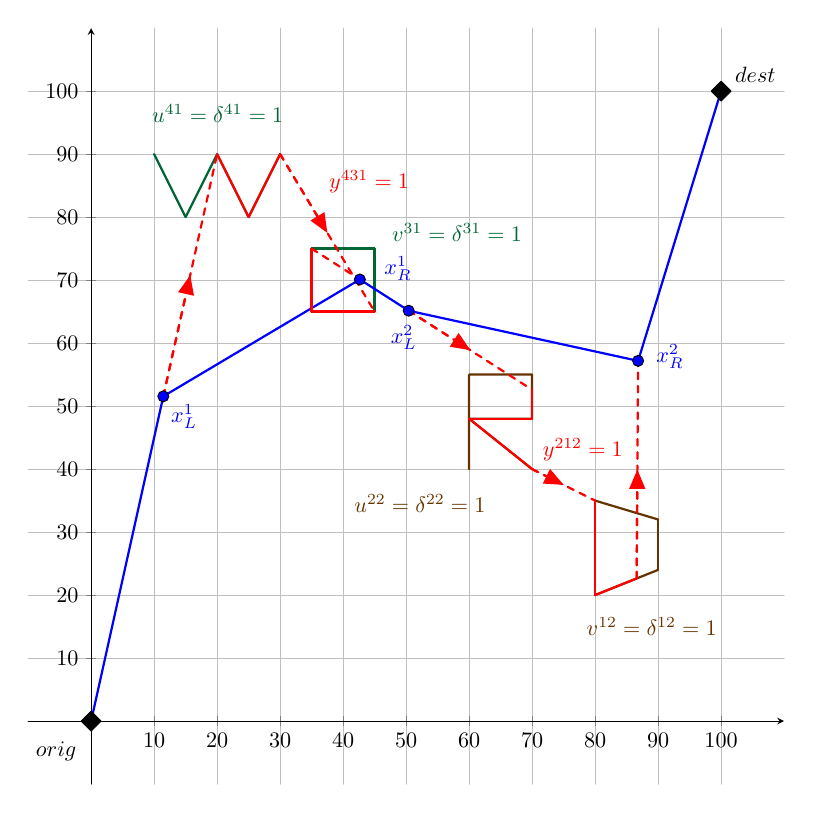
\begin{tikzpicture}[line cap=round,line join=round,>=triangle 45,x=1cm,y=1cm, scale = 0.8]
\begin{axis}[
x=0.1cm,y=0.1cm,
axis lines=middle,
ymajorgrids=true,
xmajorgrids=true,
xmin=-10,
xmax=110,
ymin=-10,
ymax=110,
xtick={0,10,...,100},
ytick={0,10,...,100},]
%\clip(-51.87275387205345,-19.48294075374569) rectangle (135.90040875888684,125.1089370909846);
\draw [line width=1pt,color=qqwwtt] (10,90)-- (15,80)-- (20,90)-- (25,80)-- (30,90);
\draw [line width=1pt] (35,75)-- (35,65);
\draw [line width=1pt] (35,65)-- (45,65);
\draw [line width=1pt,color=qqwwtt] (45,65)-- (45,75);
\draw [line width=1pt,color=qqwwtt] (45,75)-- (35,75);
\draw [line width=1pt,color=wwttqq] (60,40)-- (60,55)-- (70,55)-- (70,48)-- (60,48)-- (70,40);
\draw [line width=1pt] (80,35)-- (80,20);
\draw [line width=1pt,color=wwttqq] (80,20)-- (90,24);
\draw [line width=1pt,color=wwttqq] (90,24)-- (90,32);
\draw [line width=1pt,color=wwttqq] (90,32)-- (80,35);
\draw (-10,-2) node[anchor=north west] {$\bm{orig}$};
\draw (101,105) node[anchor=north west] {$\bm{dest}$};
\draw [color=qqwwtt](8.45897147725058,99.14529141107357) node[anchor=north west] {\bm{$u^{41}=\delta^{41}=1$}};
\draw [color=qqwwtt](46.53179129265427,80.1934233173285) node[anchor=north west] {\bm{$v^{31}=\delta^{31}=1$}};
\draw [color=wwttqq](40.55585724578162,37.26562117671086) node[anchor=north west] {\bm{$u^{22}=\delta^{22}=1$}};
\draw [color=wwttqq](77.43552748014484,17.620603501925224) node[anchor=north west] {\bm{$v^{12}=\delta^{12}=1$}};
\draw [line width=1pt,color=qqqqff] (0,0)-- (11.46,51.55);
\draw [line width=1pt,color=qqqqff] (11.46,51.55)-- (42.66,70.1);
\draw [line width=1pt,color=qqqqff] (42.66,70.1)-- (50.41,65.14);
\draw [line width=1pt,color=qqqqff] (50.41,65.14)-- (86.83,57.18);
\draw [line width=1pt,color=qqqqff] (86.83,57.18)-- (100,100);
\draw [line width=1pt,dashed,color=ffqqqq] (11.46,51.55)-- (20,90);
\draw [line width=1pt,color=ffqqqq] (20,90)-- (25,80);
\draw [line width=1pt,color=ffqqqq] (25,80)-- (30,90);
\draw [line width=1pt,dashed,color=ffqqqq] (30,90)-- (45,65);
\draw [line width=1pt,color=ffqqqq] (45,65)-- (35,65);
\draw [line width=1pt,color=ffqqqq] (35,65)-- (35,75);
\draw [line width=1pt,dashed,color=ffqqqq] (35,75)-- (42.66,70.1);
% \draw [line width=1pt,color=ffqqqq] (42.66,70.1)-- (11.46,51.55);
\draw [line width=1pt,dashed,color=ffqqqq] (50.41,65.14)-- (70,52.6);
\draw [line width=1pt,color=ffqqqq] (70,52.6)-- (70,48);
\draw [line width=1pt,color=ffqqqq] (70,48)-- (60,48);
\draw [line width=1pt,color=ffqqqq] (60,48)-- (70,40);
\draw [line width=1pt,dashed,color=ffqqqq] (70,40)-- (80,35);
\draw [line width=1pt,color=ffqqqq] (80,35)-- (80,20);
\draw [line width=1pt,color=ffqqqq] (80,20)-- (86.6,22.64);
\draw [line width=1pt,dashed,color=ffqqqq] (86.6,22.64)-- (86.83,57.18);
\draw [->,line width=1pt,dashed,color=ffqqqq] (11.46,51.55) -- (15.73,70.775);
\draw [->,line width=1pt,dashed,color=ffqqqq] (50.41,65.14) -- (60.205,58.87);
\draw [->,line width=1pt,dashed,color=ffqqqq] (86.5971,22.6388) -- (86.715,39.91);
\draw [->,line width=1pt,dashed,color=ffqqqq] (30,90) -- (37.5,77.5);
\draw [->,line width=1pt,dashed,color=ffqqqq] (70,40) -- (75,37.5);
\draw [color=ffqqqq](36.54173818934138,88.70826534025115) node[anchor=north west] {\bm{$y^{431}=1$}};
\draw [color=ffqqqq](70.47421968887281,46.158736277919324) node[anchor=north west] {\bm{$y^{212}=1$}};
\begin{scriptsize}
\draw [fill=black] (0,0) ++(-4.5pt,0 pt) -- ++(4.5pt,4.5pt)--++(4.5pt,-4.5pt)--++(-4.5pt,-4.5pt)--++(-4.5pt,4.5pt);
\draw [fill=black] (100,100) ++(-4.5pt,0 pt) -- ++(4.5pt,4.5pt)--++(4.5pt,-4.5pt)--++(-4.5pt,-4.5pt)--++(-4.5pt,4.5pt);
\draw [fill=qqqqff] (11.46,51.55) circle (2.5pt);
\draw [color=qqqqff](11.46,51.55) node[anchor=north west] {\bm{$x_L^1$}};
\draw [fill=qqqqff] (42.66,70.1) circle (2.5pt);
\draw [color=qqqqff] (45.33,75.04) node[anchor=north west]{$\bm{x_R^1}$};
\draw [fill=qqqqff] (50.41,65.14) circle (2.5pt);
\draw [color=qqqqff] (46.33,64.04) node[anchor=north west]{$\bm{x_L^2}$};
\draw [fill=qqqqff] (86.83,57.18) circle (2.5pt);
\draw [color=qqqqff] (88.5,61.04) node[anchor=north west]{$\bm{x_R^2}$};
\end{scriptsize}
\end{axis}
\end{tikzpicture}
\caption{Solution provided by the matheuristic.}
\label{fig:Fig7}
\end{figure}